\section{Results}

\subsection{Heatmap}

The expression values of all 17,381 probesets across all 9 samples were analysed
by the \lstinline|heatmap.R| script to produce a false-color representation of
expression value z-scores on a yellow-red scale with additional dendrograms of
distances on both the sample and the probeset axis (see figure
\ref{fig:heatmap}). The filtering process implemented in R, which is similar to
our own statistical analysis and filtering, results in 689 probesets above the
threshold of 2fold over- or underexpression.

The heatmap provides a general overview of the dataset and confirms the
functionality of all processing steps up to this point. Additionally it can be
used to compare the output of our implementations for z-score and p value
calculation as these were implemented separately in R and Python.

Unfortunately the very high number of probesets combined with the limited
resolution of the output figure make it impossible to read the individual gene
IDs at the bottom of the figure along the x axis, which are needed for
interpretation of the dendrogram clusters depicted above figure. However, the
dendrogram of the 9 tissues used in our analysis remains interpretable and shows
tissue \#4 (GSM433779) and \#8 (GSM433783) as having a different expression
pattern than the rest. In tissue \#4 several clusters of genes (depicted in red,
left half of heatmap) are up-regulated while a large contiguous area (depicted
in yellow, third quarter of heatmap) is down-regulated. The pattern of \#8 is a
bit different from that of \#4. Here the over-expressed and down-regulated
regions are a bit shifted and shorter but roughly in the same regions. Neither
of these special patterns within \#4 and \#8 can be found in any of the other
tissues, which warrants a closer examination of tissue GSM433779 and GSM433783.

\begin{figure}[h]
 \centering
 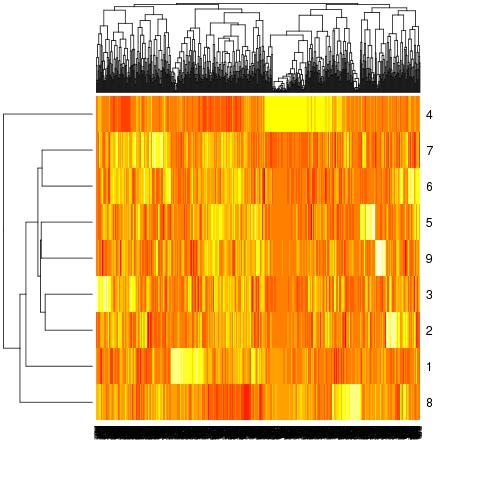
\includegraphics[scale=0.60,keepaspectratio=true]{../R/heatmap.jpg}
 % heatmap.jpg: 480x480 pixel, 72dpi, 16.93x16.93 cm, bb=0 0 480 480
 \caption{Heatmap of expression values; color values range from low (yellow) to
high (red) expression; numbers correspond to the following tissue samples: 1 =
GSM433776, 2 = GSM433777, 3 = GSM433778, 4 = GSM433779, 5 = GSM433780, 6 =
GSM433781, 7 = GSM433782, 8 = GSM433783, 9 = GSM433784; the x-axis shows
clustering of 689 probesets by similarity of expression values while the y-axis
shows clustering of 9 tissues by similarity of expression values}
 \label{fig:heatmap}
\end{figure}

\subsection{Exploration of enriched Gene Sets}

\subsubsection{Fisher's exact test}

To all tissues the Fischer's exact test was applied to gene sets correlating to
the KEGG pathways and a GO term gene set database. For both gene set classes we
calculated a list of the 30 sets with the lowest p values among all tissues.
Many cancer unrelated pathways were found in the list like ALZHEIMERS DISEASE,
LYSOSOME, ECM RECEPTOR INTERACTION, TYPE I DIABETES MELLITUS, PARKINSONS
DISEASE, KHUNTINGTONS DISEASE. Most of them were connected to tissue GSM433779.
Some of the cancer related gene sets within the list were KEGG FOCAL ADHESION,
PATHWAYS IN CANCER, SMALL CELL LUNG CANCER and MELANOGENESIS. All four were
found in tissue GSM433783, GSM433782 and GSM433781, but only tissue GSM433783
contained all of them.


\begin{center}
\small
\renewcommand{\tablename}{\normalsize Table}    % sorgt für normale Überschrift auch bei kleinen longtables
% \renewcommand{\arraystretch}{1.5}     % erweitert Zeilenabstand in Tabellen!
\begin{longtable}[tbp]{lll}
\caption[Top 30 KEGG pathways]{\label{tab:top30kegg}Top 30 KEGG pathways as
produced by Fisher exact test for gene set enrichment analysis; the KEGG term
KEGG\_ARRHYTHMO\-GENIC\_RIGHT\_VENTRICULAR\_CARDIO\-MYOPATHY\_ARVC has been
shortened to KEGG\_ARVC to fit the page}\\
\textbf{tissue} & \textbf{KEGG pathway} & \textbf{p value} \\ \toprule \endfirsthead
\textbf{tissue} & \textbf{KEGG pathway} & \textbf{p value} \\ \toprule \endhead
\multicolumn{3}{r}{\tiny{continued on next page}} \endfoot
\endlastfoot
GSM433783 & KEGG\_FOCAL\_ADHESION & $2.0477 \cdot 10^{-2}$ \\
GSM433779 & KEGG\_ANTIGEN\_PROCESSING\_AND\_PRESENTATION & $4.2654 \cdot 10^{-2}$ \\
GSM433779 & KEGG\_ALZHEIMERS\_DISEASE & $6.9883 \cdot 10^{-2}$ \\
GSM433779 & KEGG\_LYSOSOME & $7.2256 \cdot 10^{-2}$ \\
GSM433783 & KEGG\_ECM\_RECEPTOR\_INTERACTION & $8.2122 \cdot 10^{-2}$ \\
GSM433783 & KEGG\_LYSOSOME & $1.1015 \cdot 10^{-1}$ \\
GSM433783 & KEGG\_PATHWAYS\_IN\_CANCER & $1.2493 \cdot 10^{-1}$ \\
GSM433779 & KEGG\_OOCYTE\_MEIOSIS & $1.6001 \cdot 10^{-1}$ \\
GSM433779 & KEGG\_NOD\_LIKE\_RECEPTOR\_SIGNALING\_PATHWAY & $1.6001 \cdot 10^{-1}$ \\
GSM433779 & KEGG\_PROGESTERONE\_MEDIATED\_OOCYTE\_MATURATION & $1.6001 \cdot 10^{-1}$ \\
GSM433779 & KEGG\_TYPE\_I\_DIABETES\_MELLITUS & $1.6001 \cdot 10^{-1}$ \\
GSM433779 & KEGG\_GRAFT\_VERSUS\_HOST\_DISEASE & $1.6001 \cdot 10^{-1}$ \\
GSM433779 & KEGG\_OXIDATIVE\_PHOSPHORYLATION & $1.6211 \cdot 10^{-1}$ \\
GSM433779 & KEGG\_HEMATOPOIETIC\_CELL\_LINEAGE & $1.6211 \cdot 10^{-1}$ \\
GSM433782 & KEGG\_PATHWAYS\_IN\_CANCER & $1.8626 \cdot 10^{-1}$ \\
GSM433783 & KEGG\_ADHERENS\_JUNCTION & $1.9733 \cdot 10^{-1}$ \\
GSM433779 & KEGG\_PARKINSONS\_DISEASE & $1.9818 \cdot 10^{-1}$ \\
GSM433779 & KEGG\_HUNTINGTONS\_DISEASE & $1.9818 \cdot 10^{-1}$ \\
GSM433779 & KEGG\_TOLL\_LIKE\_RECEPTOR\_SIGNALING\_PATHWAY & $2.0817 \cdot 10^{-1}$ \\
GSM433783 & KEGG\_AXON\_GUIDANCE & $2.1736 \cdot 10^{-1}$ \\
GSM433781 & KEGG\_PATHWAYS\_IN\_CANCER & $2.3590 \cdot 10^{-1}$ \\
GSM433783 & KEGG\_SMALL\_CELL\_LUNG\_CANCER & $2.3938 \cdot 10^{-1}$ \\
GSM433783 & KEGG\_ARVC & $2.6359 \cdot 10^{-1}$ \\
GSM433779 & KEGG\_B\_CELL\_RECEPTOR\_SIGNALING\_PATHWAY & $2.7070 \cdot 10^{-1}$ \\
GSM433779 & KEGG\_ASTHMA & $2.7070 \cdot 10^{-1}$ \\
GSM433779 & KEGG\_AUTOIMMUNE\_THYROID\_DISEASE & $2.7070 \cdot 10^{-1}$ \\
GSM433779 & KEGG\_ALLOGRAFT\_REJECTION & $2.7070 \cdot 10^{-1}$ \\
GSM433776 & KEGG\_WNT\_SIGNALING\_PATHWAY & $2.7829 \cdot 10^{-1}$ \\
GSM433783 & KEGG\_WNT\_SIGNALING\_PATHWAY & $2.9020 \cdot 10^{-1}$ \\
GSM433783 & KEGG\_MELANOGENESIS & $2.9020 \cdot 10^{-1}$
\end{longtable}
\end{center}

The p-Values for the GO terms were calculated as required, but we decided to
disregard those results for the discussion as their usefulness is highly
doubtful. The file \verb|c5.all.v3.1.entrez.gmt| only provides a single GO term
without any GO-ID or additional GO terms complementing the given single GO term.
Any GO term for a set is either a \textbf{single} cellular component, biological
process or molecular function. Thus a result like ``NUCLEUS'' without any
additional terms might point to anything from nucleus transport protein over
signal molecule to cancer associated proteins like p53. The only interesting
result might have been to find a lot of biological processes or molecular
functions associated with cancer like behavior, but all top scoring GO terms
stood for not cancer associated cellular components or biological processes. 

\begin{center}
\small
\renewcommand{\tablename}{\normalsize Table}    % sorgt für normale Überschrift auch bei kleinen longtables
% \renewcommand{\arraystretch}{1.5}     % erweitert Zeilenabstand in Tabellen!
\begin{longtable}[tbp]{lll}
\caption[Top 30 GO terms]{\label{tab:top30go}Top 30 GO terms as produced by Fisher exact test for gene set enrichment analysis}\\
\textbf{tissue} & \textbf{GO term} & \textbf{p value} \\ \toprule \endfirsthead
\textbf{tissue} & \textbf{GO term} & \textbf{p value} \\ \toprule \endhead
\multicolumn{3}{r}{\tiny{continued on next page}} \endfoot
\endlastfoot
GSM433776 & ANATOMICAL\_STRUCTURE\_DEVELOPMENT & $4.1484 \cdot 10^{-3}$ \\
GSM433776 & MULTICELLULAR\_ORGANISMAL\_DEVELOPMENT & $6.0841 \cdot 10^{-3}$ \\
GSM433776 & ORGAN\_DEVELOPMENT & $1.0661 \cdot 10^{-2}$ \\
GSM433776 & SYSTEM\_DEVELOPMENT & $1.4116 \cdot 10^{-2}$ \\
GSM433779 & NUCLEUS & $1.6135 \cdot 10^{-2}$ \\
GSM433784 & MEMBRANE & $1.6535 \cdot 10^{-2}$ \\
GSM433776 & EXTRACELLULAR\_REGION & $2.4333 \cdot 10^{-2}$ \\
GSM433779 & NUCLEAR\_PART & $3.2700  \cdot 10^{-2}$ \\
GSM433776 & ANATOMICAL\_STRUCTURE\_MORPHOGENESIS & $3.3341 \cdot 10^{-2}$ \\
GSM433784 & MEMBRANE\_PART & $3.3632 \cdot 10^{-2}$ \\
GSM433776 & TRANSMEMBRANE\_RECEPTOR\_ACTIVITY & $3.6945 \cdot 10^{-2}$ \\
GSM433784 & PLASMA\_MEMBRANE & $6.2403 \cdot 10^{-2}$ \\
GSM433784 & INTRINSIC\_TO\_MEMBRANE & $6.9048 \cdot 10^{-2}$ \\
GSM433784 & INTEGRAL\_TO\_MEMBRANE & $6.9048 \cdot 10^{-2}$ \\
GSM433779 & ORGANELLE\_LUMEN & $7.2481 \cdot 10^{-2}$ \\
GSM433779 & ENVELOPE & $7.2481 \cdot 10^{-2}$ \\
GSM433779 & ORGANELLE\_ENVELOPE & $7.2481 \cdot 10^{-2}$ \\
GSM433779 & MEMBRANE\_ENCLOSED\_LUMEN & $7.2481 \cdot 10^{-2}$ \\
GSM433776 & LIPID\_METABOLIC\_PROCESS & $7.5447 \cdot 10^{-2}$ \\
GSM433784 & PROTEIN\_METABOLIC\_PROCESS & $7.6362 \cdot 10^{-2}$ \\
GSM433776 & INTRINSIC\_TO\_MEMBRANE & $8.0530 \cdot 10^{-2}$ \\
GSM433776 & INTEGRAL\_TO\_MEMBRANE & $8.0530 \cdot 10^{-2}$ \\
GSM433776 & EXTRACELLULAR\_REGION\_PART & $8.1680 \cdot 10^{-2}$ \\
GSM433779 & MITOCHONDRION & $8.6676 \cdot 10^{-2}$ \\
GSM433776 & CELLULAR\_LOCALIZATION & $9.2386 \cdot 10^{-2}$ \\
GSM433784 & CELLULAR\_MACROMOLECULE\_METABOLIC\_PROCESS & $9.3255 \cdot 10^{-2}$ \\
GSM433784 & CELLULAR\_PROTEIN\_METABOLIC\_PROCESS & $9.9635 \cdot 10^{-2}$ \\
GSM433783 & PROTEIN\_DIMERIZATION\_ACTIVITY & $9.9893 \cdot 10^{-2}$ \\
GSM433776 & ENDOPLASMIC\_RETICULUM & $1.0221 \cdot 10^{-1}$ \\
GSM433776 & ESTABLISHMENT\_OF\_CELLULAR\_LOCALIZATION & $1.0221 \cdot 10^{-1}$
\end{longtable}
\end{center}



\subsubsection{Gene Set Enrichment Analysis}
The Gene Set Enrichment Analysis initially rejects 174 of the 186 given gene
sets, leaving 12 sets that show significant deregulation among the nine given
cancer cell lines.

\begin{table}[htp]
 \centering
  \caption[Pathways selected by GSEA]{\label{tab:gsea12}List of pathways used in GSEA}
 \begin{tabular}{l}
\textbf{list of selected pathways} \\ \hline
KEGG\_MAPK\_SIGNALING\_PATHWAY   \\
KEGG\_CYTOKINE\_CYTOKINE\_RECEPTOR\_INTERACTION   \\
KEGG\_LYSOSOME   \\
KEGG\_AXON\_GUIDANCE   \\
KEGG\_FOCAL\_ADHESION   \\
KEGG\_ECM\_RECEPTOR\_INTERACTION   \\
KEGG\_CELL\_ADHESION\_MOLECULES\_CAMS   \\
KEGG\_ADHERENS\_JUNCTION   \\
KEGG\_REGULATION\_OF\_ACTIN\_CYTOSKELETON   \\
KEGG\_ALZHEIMERS\_DISEASE   \\
KEGG\_PATHWAYS\_IN\_CANCER   \\
KEGG\_SMALL\_CELL\_LUNG\_CANCER
  \end{tabular}
\end{table}

The results of Fisher's exact test indicated that in tissue GSM433783 genes
correlated with oncogenic pathways were deregulated compared to the other cell
lines. For that reason the GSEA results for GSM433783 were checked in more
detail. The GSEA output showed the focal adhesion, small cell lung cancer and
pathways in cancer pathways to be relevant again. Their p-Values were among the
lowest. Except the lysosome pathways all other findings were regulated down
compared to the rest, as can be seen from the negative enrichment scores.

\begin{table}[htp]
 \centering
  \caption[GSEA output for 83]{\label{tab:gsea_res_83}GSEA enrichment scores and
p-values for sample GSM433783 compared to the remaining tissues}
 \begin{tabular}{l c c}
\textbf{NAME} & \textbf{ES}  & \textbf{NOM p-val}  \\ \hline
KEGG\_FOCAL\_ADHESION & -0.27030912 & 0.00998004 \\
KEGG\_REGULATION\_OF\_ACTIN\_CYTOSKELETON & -0.28983307 & 0.052738335  \\
KEGG\_ADHERENS\_JUNCTION & -0.3143161 & 0.055666003  \\
KEGG\_SMALL\_CELL\_LUNG\_CANCER & -0.31651652 & 0.065737054 \\
KEGG\_PATHWAYS\_IN\_CANCER & -0.20688379 & 0.083657585  \\
KEGG\_ALZHEIMERS\_DISEASE & -0.29491496 & 0.09343936 \\
KEGG\_MAPK\_SIGNALING\_PATHWAY & -0.25829262 & 0.12627292 \\
KEGG\_ECM\_RECEPTOR\_INTERACTION & -0.22219512 & 0.16763006  \\
KEGG\_CYTOKINE\_CYTOKINE\_RECEPTOR\_INTER. & -0.20512007 & 0.37669903 \\
KEGG\_CELL\_ADHESION\_MOLECULES\_CAMS & -0.16316189 & 0.6065259  \\
KEGG\_AXON\_GUIDANCE & -0.16156015 & 0.77734375  \\
KEGG\_LYSOSOME & 0.22209951 & 0.2090164 
  \end{tabular}
\end{table}






% original tables with unabridged float values, keep as backup!

%
% \begin{center}
% \small
% \renewcommand{\tablename}{\normalsize Table}    % sorgt für normale Überschrift auch bei kleinen longtables
% % \renewcommand{\arraystretch}{1.5}     % erweitert Zeilenabstand in Tabellen!
% \begin{longtable}[tbp]{lll}
% \caption[Top 30 GO terms]{\label{tab:top30go}Top 30 GO terms as produced by Fisher exact test for gene set enrichment analysis}\\
% \textbf{tissue} & \textbf{GO term} & \textbf{p value} \\ \toprule \endfirsthead
% \textbf{tissue} & \textbf{GO term} & \textbf{p value} \\ \toprule \endhead
% \multicolumn{3}{r}{\tiny{continued on next page}} \endfoot
% \endlastfoot
% GSM433776 & ANATOMICAL\_STRUCTURE\_DEVELOPMENT & 0.0041484199593353208 \\
% GSM433776 & MULTICELLULAR\_ORGANISMAL\_DEVELOPMENT & 0.0060840851876180603 \\
% GSM433776 & ORGAN\_DEVELOPMENT & 0.010660750298390706 \\
% GSM433776 & SYSTEM\_DEVELOPMENT & 0.01411589211200644 \\
% GSM433779 & NUCLEUS & 0.01613517522699693 \\
% GSM433784 & MEMBRANE & 0.016535017545091402 \\
% GSM433776 & EXTRACELLULAR\_REGION & 0.024333384123555228 \\
% GSM433779 & NUCLEAR\_PART & 0.032699651620653768 \\
% GSM433776 & ANATOMICAL\_STRUCTURE\_MORPHOGENESIS & 0.033340640756852828 \\
% GSM433784 & MEMBRANE\_PART & 0.033632016582334494 \\
% GSM433776 & TRANSMEMBRANE\_RECEPTOR\_ACTIVITY & 0.036945034352169094 \\
% GSM433784 & PLASMA\_MEMBRANE & 0.062403042186338083 \\
% GSM433784 & INTRINSIC\_TO\_MEMBRANE & 0.069048161249155901 \\
% GSM433784 & INTEGRAL\_TO\_MEMBRANE & 0.069048161249155901 \\
% GSM433779 & ORGANELLE\_LUMEN & 0.072480776571242189 \\
% GSM433779 & ENVELOPE & 0.072480776571242189 \\
% GSM433779 & ORGANELLE\_ENVELOPE & 0.072480776571242189 \\
% GSM433779 & MEMBRANE\_ENCLOSED\_LUMEN & 0.072480776571242189 \\
% GSM433776 & LIPID\_METABOLIC\_PROCESS & 0.075447171713395392 \\
% GSM433784 & PROTEIN\_METABOLIC\_PROCESS & 0.076361987668977907 \\
% GSM433776 & INTRINSIC\_TO\_MEMBRANE & 0.080530451780604778 \\
% GSM433776 & INTEGRAL\_TO\_MEMBRANE & 0.080530451780604778 \\
% GSM433776 & EXTRACELLULAR\_REGION\_PART & 0.081680250423794856 \\
% GSM433779 & MITOCHONDRION & 0.086675770578363939 \\
% GSM433776 & CELLULAR\_LOCALIZATION & 0.092386170664946171 \\
% GSM433784 & CELLULAR\_MACROMOLECULE\_METABOLIC\_PROCESS & 0.093255085523524142 \\
% GSM433784 & CELLULAR\_PROTEIN\_METABOLIC\_PROCESS & 0.099635155036457812 \\
% GSM433783 & PROTEIN\_DIMERIZATION\_ACTIVITY & 0.099892995593273665 \\
% GSM433776 & ENDOPLASMIC\_RETICULUM & 0.10220795625052388 \\
% GSM433776 & ESTABLISHMENT\_OF\_CELLULAR\_LOCALIZATION & 0.10220795625052388
% \end{longtable}
% \end{center}
%
% \begin{center}
% \small
% \renewcommand{\tablename}{\normalsize Table}    % sorgt für normale Überschrift auch bei kleinen longtables
% % \renewcommand{\arraystretch}{1.5}     % erweitert Zeilenabstand in Tabellen!
% \begin{longtable}[tbp]{lll}
% \caption[Top 30 KEGG pathways]{\label{tab:top30kegg}Top 30 KEGG pathways as produced by Fisher exact test for gene set enrichment analysis}\\
% \textbf{tissue} & \textbf{KEGG pathway} & \textbf{p value} \\ \toprule \endfirsthead
% \textbf{tissue} & \textbf{KEGG pathway} & \textbf{p value} \\ \toprule \endhead
% \multicolumn{3}{r}{\tiny{continued on next page}} \endfoot
% \endlastfoot
% GSM433783 & KEGG\_FOCAL\_ADHESION & 0.02047735026470849 \\
% GSM433779 & KEGG\_ANTIGEN\_PROCESSING\_AND\_PRESENTATION & 0.04265445885777662 \\
% GSM433779 & KEGG\_ALZHEIMERS\_DISEASE & 0.069883295166020432 \\
% GSM433779 & KEGG\_LYSOSOME & 0.07225594581272575 \\
% GSM433783 & KEGG\_ECM\_RECEPTOR\_INTERACTION & 0.082121923992907797 \\
% GSM433783 & KEGG\_LYSOSOME & 0.11014691235937486 \\
% GSM433783 & KEGG\_PATHWAYS\_IN\_CANCER & 0.12492697216103343 \\
% GSM433779 & KEGG\_OOCYTE\_MEIOSIS & 0.16001465453063529 \\
% GSM433779 & KEGG\_NOD\_LIKE\_RECEPTOR\_SIGNALING\_PATHWAY & 0.16001465453063529 \\
% GSM433779 & KEGG\_PROGESTERONE\_MEDIATED\_OOCYTE\_MATURATION & 0.16001465453063529 \\
% GSM433779 & KEGG\_TYPE\_I\_DIABETES\_MELLITUS & 0.16001465453063529 \\
% GSM433779 & KEGG\_GRAFT\_VERSUS\_HOST\_DISEASE & 0.16001465453063529 \\
% GSM433779 & KEGG\_OXIDATIVE\_PHOSPHORYLATION & 0.16211214570311805 \\
% GSM433779 & KEGG\_HEMATOPOIETIC\_CELL\_LINEAGE & 0.16211214570311805 \\
% GSM433782 & KEGG\_PATHWAYS\_IN\_CANCER & 0.1862581213728749 \\
% GSM433783 & KEGG\_ADHERENS\_JUNCTION & 0.19733310104478013 \\
% GSM433779 & KEGG\_PARKINSONS\_DISEASE & 0.19817917807771401 \\
% GSM433779 & KEGG\_HUNTINGTONS\_DISEASE & 0.19817917807771401 \\
% GSM433779 & KEGG\_TOLL\_LIKE\_RECEPTOR\_SIGNALING\_PATHWAY & 0.20817144579873428 \\
% GSM433783 & KEGG\_AXON\_GUIDANCE & 0.21735708183823202 \\
% GSM433781 & KEGG\_PATHWAYS\_IN\_CANCER & 0.23590073177218074 \\
% GSM433783 & KEGG\_SMALL\_CELL\_LUNG\_CANCER & 0.23937691692654692 \\
% GSM433783 & KEGG\_ARRHYTHMOGENIC\_RIGHT\_VENTRICULAR\_CARDIOMYOPATHY\_ARVC & 0.26358795909527777 \\
% GSM433779 & KEGG\_B\_CELL\_RECEPTOR\_SIGNALING\_PATHWAY & 0.27070203217941369 \\
% GSM433779 & KEGG\_ASTHMA & 0.27070203217941369 \\
% GSM433779 & KEGG\_AUTOIMMUNE\_THYROID\_DISEASE & 0.27070203217941369 \\
% GSM433779 & KEGG\_ALLOGRAFT\_REJECTION & 0.27070203217941369 \\
% GSM433776 & KEGG\_WNT\_SIGNALING\_PATHWAY & 0.27828568311373758 \\
% GSM433783 & KEGG\_WNT\_SIGNALING\_PATHWAY & 0.29020433281487196 \\
% GSM433783 & KEGG\_MELANOGENESIS & 0.29020433281487196
% \end{longtable}
% \end{center}


\subsection{Visualization of selected pathways with BiNA}

The three pathways identified both by Fischer's exact test and GSEA (``Pathways
in cancer'', ``Small cell lung cancer'' and ``Focal adhesion'') were further
analyzed by using the raw expression values and mapping them onto the pathway
illustrations using the tool BiNA (Bioinformatic Network Analysis). By visual
inspection of the three pathways, it is possible to identify considerably
down-regulated genes within GSM433783 in comparison to the other tissues.
``Pathways in cancer'' and ``Small cell lung cancer'' contain exactly the same
two deregulated genes: \textit{myc} and \textit{cdk2} while in ``focal
adhesion'' \textit{catenin}. All three genes are down-regulated in comparison to
the remaining tissues. On the other hand we could not to identify any
up-regulated genes for GSM433783 in any of these pathways.

\begin{figure}[Htbp]
 \centering
 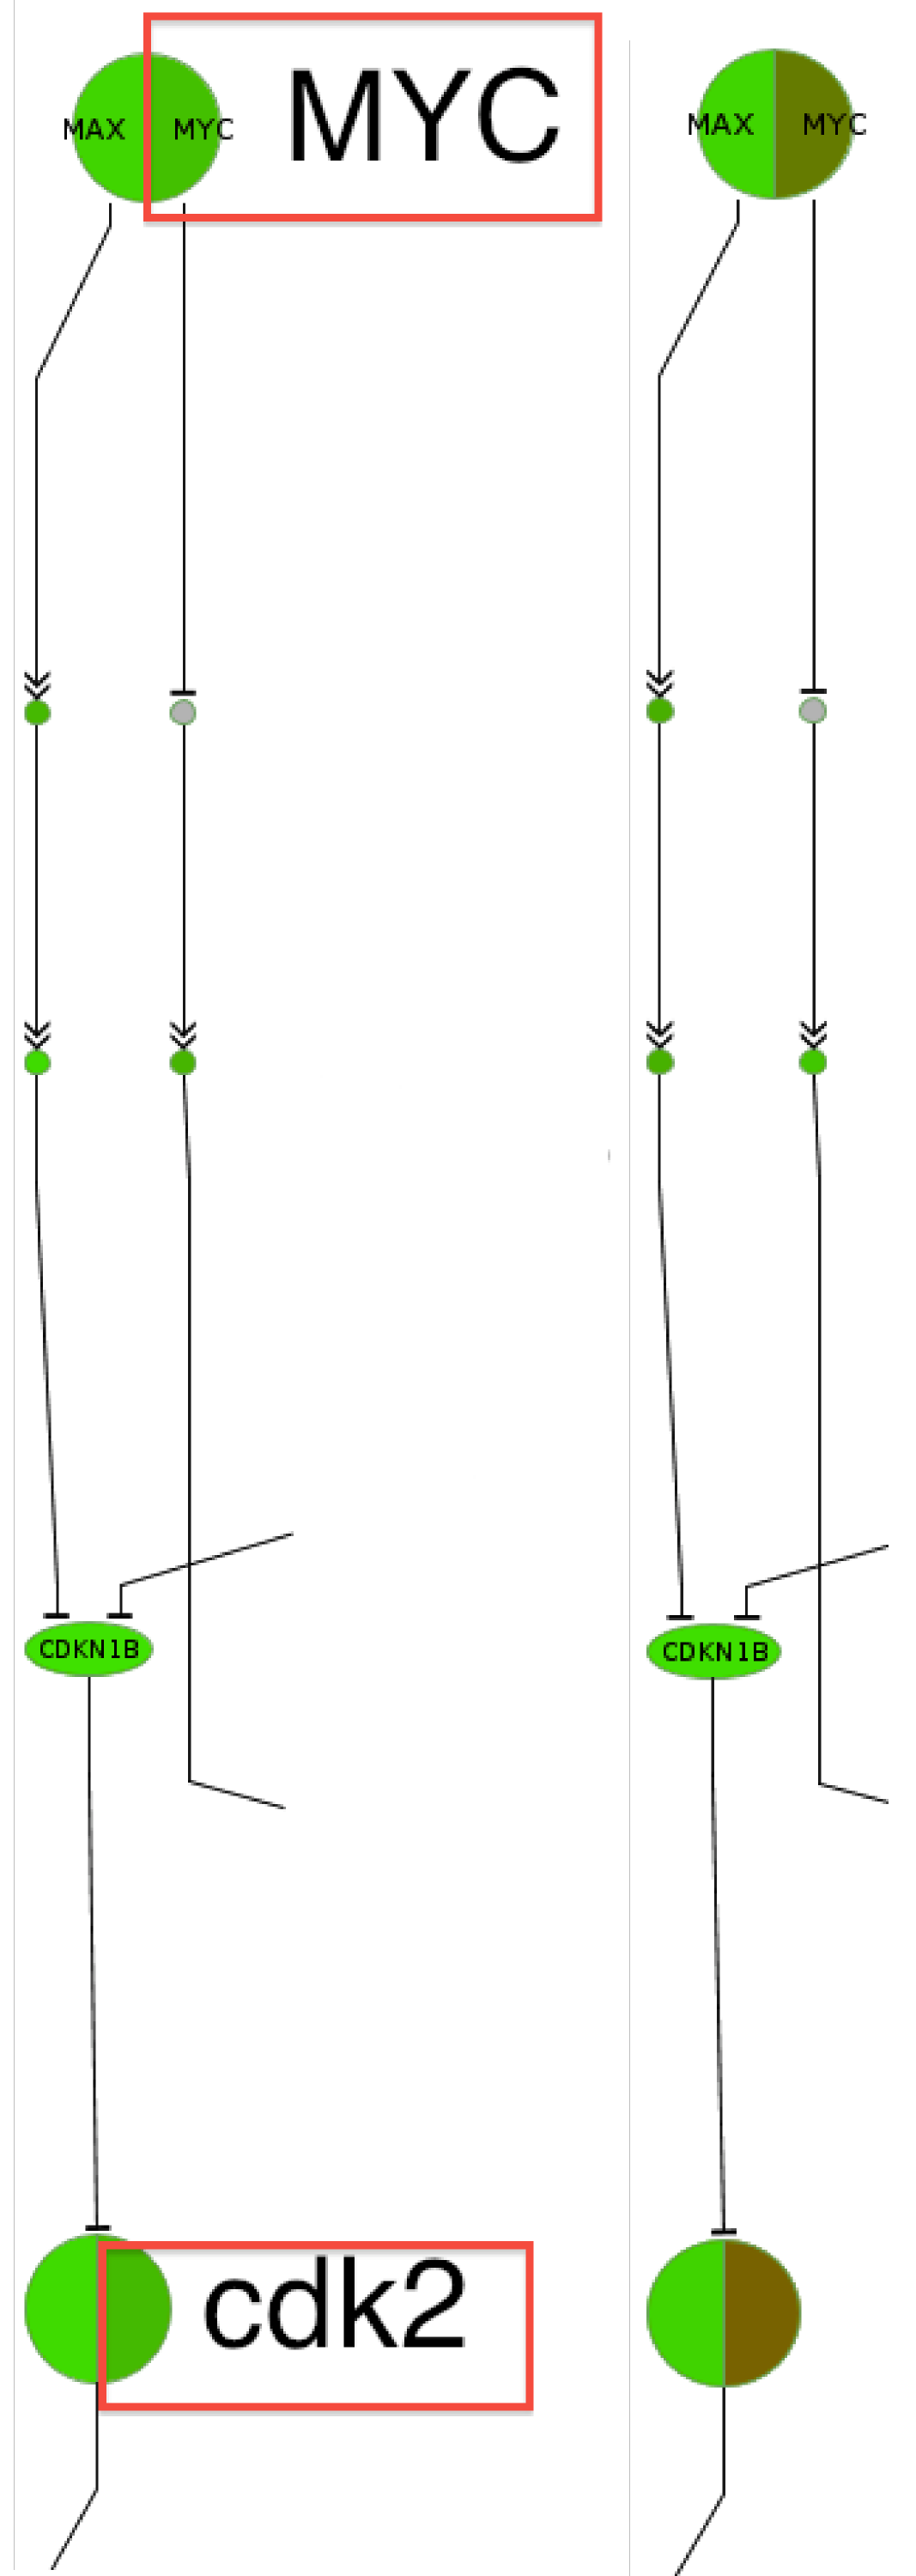
\includegraphics[scale=0.3]{./img/pinc.png}
 % pinc.png: 1067x3000 pixel, 300dpi, 9.03x25.40 cm, bb=0 0 256 720
 \caption{A small section from the KEGG pathway \textit{``Pathways in cancer''}
visualized by BiNA from the given expression values for the nine tissues. Left:
in tissue GSM433783 the two proteins \textit{myc} and \textit{cdk2} are marked
and display average expression levels as indicated by the green color of their
nodes. Right: the same section but this time the average over all remaining
samples. In average the same proteins have here significantly higher expression
levels as can be deduced from the red color for their node. All other proteins
are unchanged in comparison to GSM433783.}
 \label{fig:pathwaysincancer}
\end{figure}

% \begin{figure}[h]
% \centering
% \begin{minipage}{.4\textwidth}
%   \centering
%   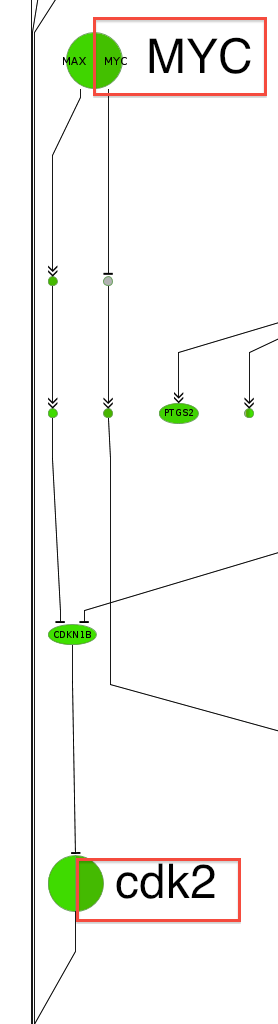
\includegraphics[width=0.5\linewidth]{p_in_cancer83.png}
% \end{minipage}
% \begin{minipage}{.4\textwidth}
%   \centering
%   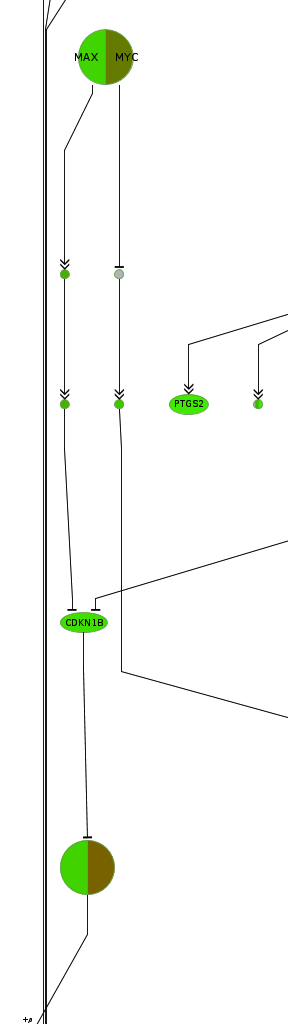
\includegraphics[width=0.5\linewidth]{p_in_cancer_avg.png}
% \end{minipage}
% \caption{A small section from the KEGG pathway \textit{``Pathways in cancer''}
% visualized by BiNA from the given expression values for the nine tissues. Left:
% in tissue GSM433783 the two proteins \textit{myc} and \textit{cdk2} are marked
% and display average expression levels as indicated by the green color of their
% nodes. Right: the same section but this time the average over all remaining
% samples. In average the same proteins have here significantly higher expression
% levels as can be deduced from the red color for their node. All other proteins
% are unchanged in comparison to GSM433783.}
% \label{fig:pathwaysincancer}
% \end{figure}

\begin{figure}[Htbp]
 \centering
 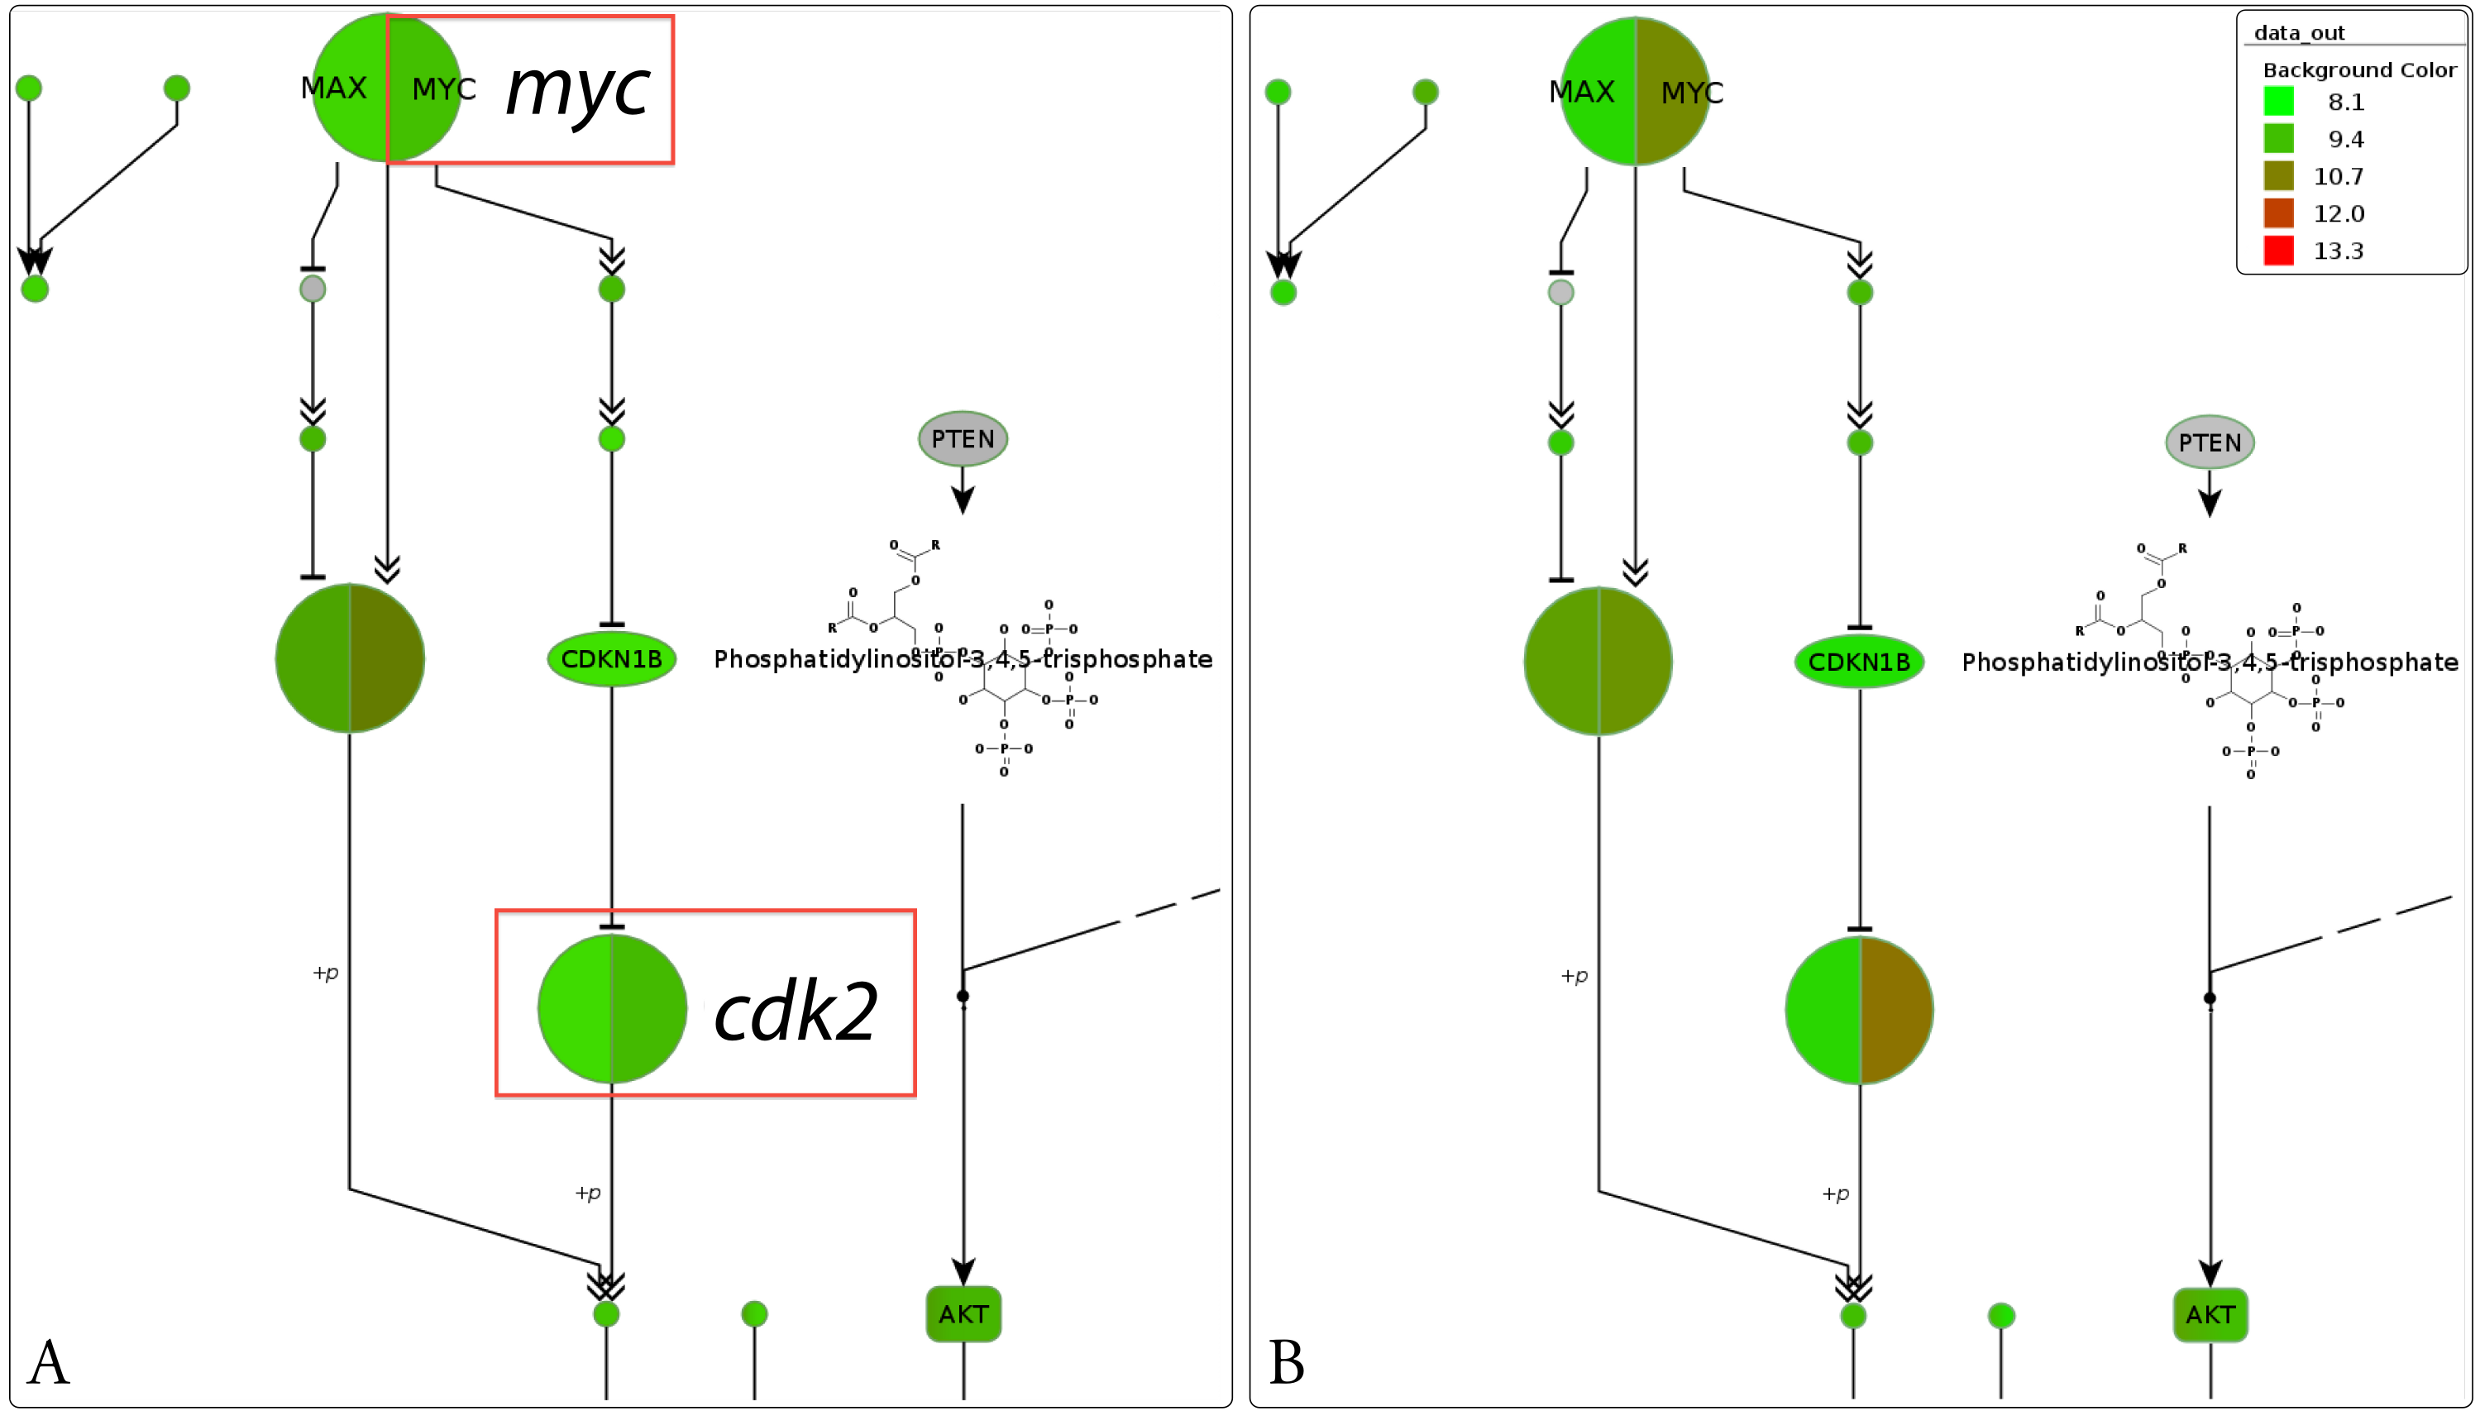
\includegraphics[scale=0.7]{./img/sclc_scaled.png}
 \caption{A section from the KEGG pathway \textit{``Small cell lung cancer''}
visualized by BiNA from the given expression values for the nine tissues. A:
in tissue GSM433783 the two proteins \textit{myc} and \textit{cdk2} are marked
and display average expression levels as indicated by the green color of their
nodes. B: the same section but this time the average over all remaining
samples. In average the same proteins have here significantly higher expression
levels as can be deduced from the red color for their node. All other proteins
are unchanged in comparison to GSM433783. This is basically the same as in the
figure of \textit{``Pathways in cancer''}, because we are looking at the same
expression values, but this time in a slightly different context.}
 \label{fig:SCLC}
\end{figure}

% \begin{figure}[h]
% \centering
% \begin{minipage}{.4\textwidth}
%   \centering
%   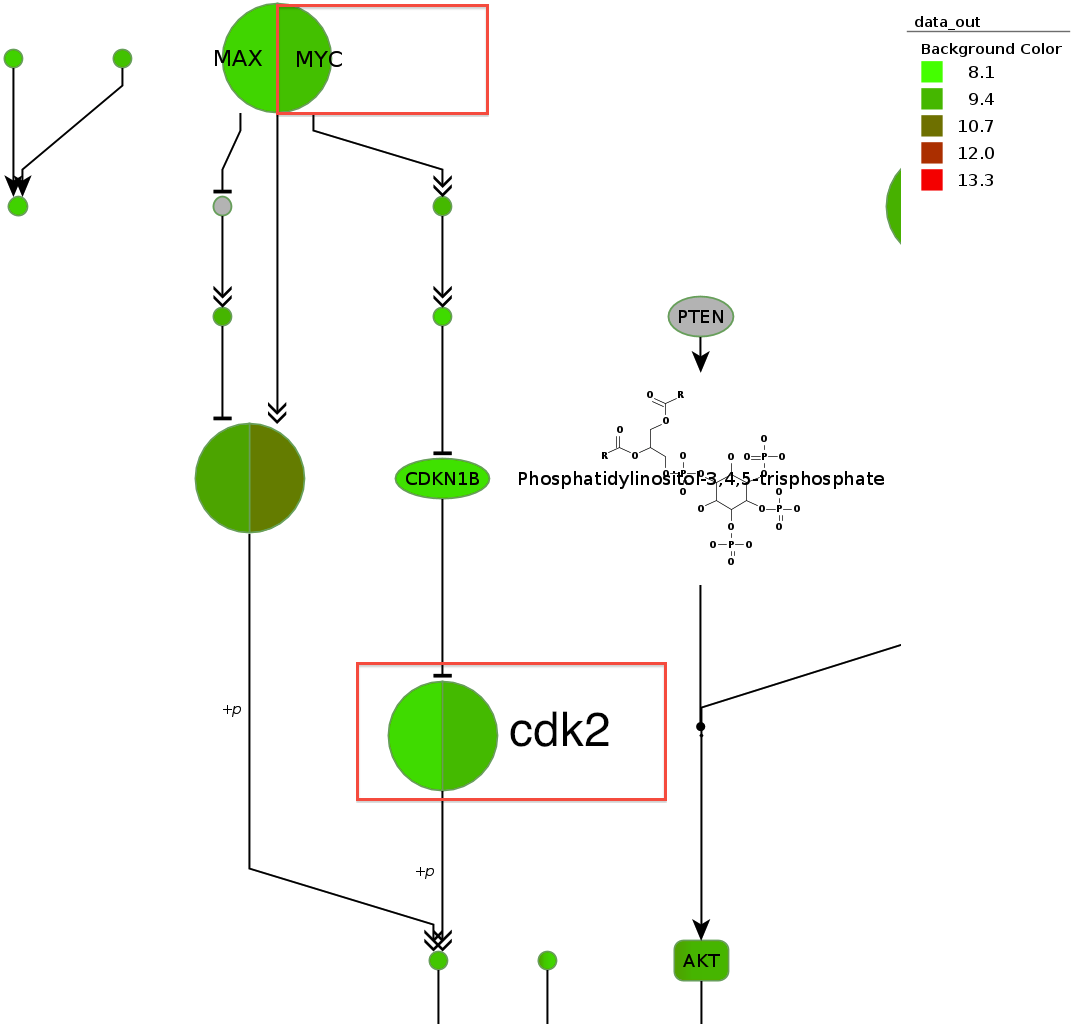
\includegraphics[width=1.2\linewidth]{p_in_SC_Lung_cancer83.png}
% \end{minipage}
% \begin{minipage}{.4\textwidth}
%   \centering
%   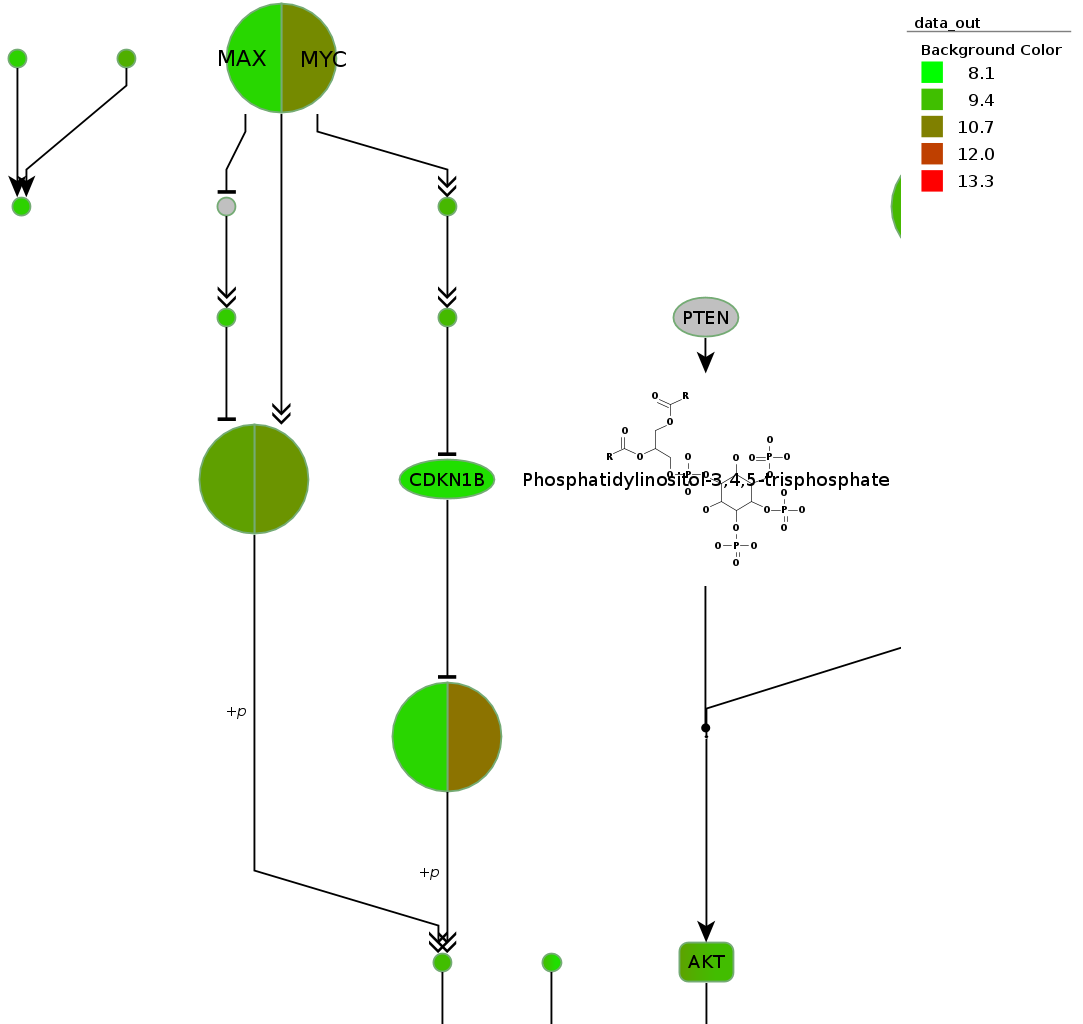
\includegraphics[width=1.2\linewidth]{p_in_SC_Lung_cancer_avg.png}
% \end{minipage}
% \caption{A section from the KEGG pathway \textit{``Small cell lung cancer''}
% visualized by BiNA from the given expression values for the nine tissues. Left:
% in tissue GSM433783 the two proteins \textit{myc} and \textit{cdk2} are marked
% and display average expression levels as indicated by the green color of their
% nodes. Right: the same section but this time the average over all remaining
% samples. In average the same proteins have here significantly higher expression
% levels as can be deduced from the red color for their node. All other proteins
% are unchanged in comparison to GSM433783. This is basically the same as in the
% figure of \textit{``Pathways in cancer''}, because we are looking at the same
% expression values, but this time in a slightly different context.}
% \label{fig:SCLC}
% \end{figure}

\begin{figure}[htbp]
 \centering
 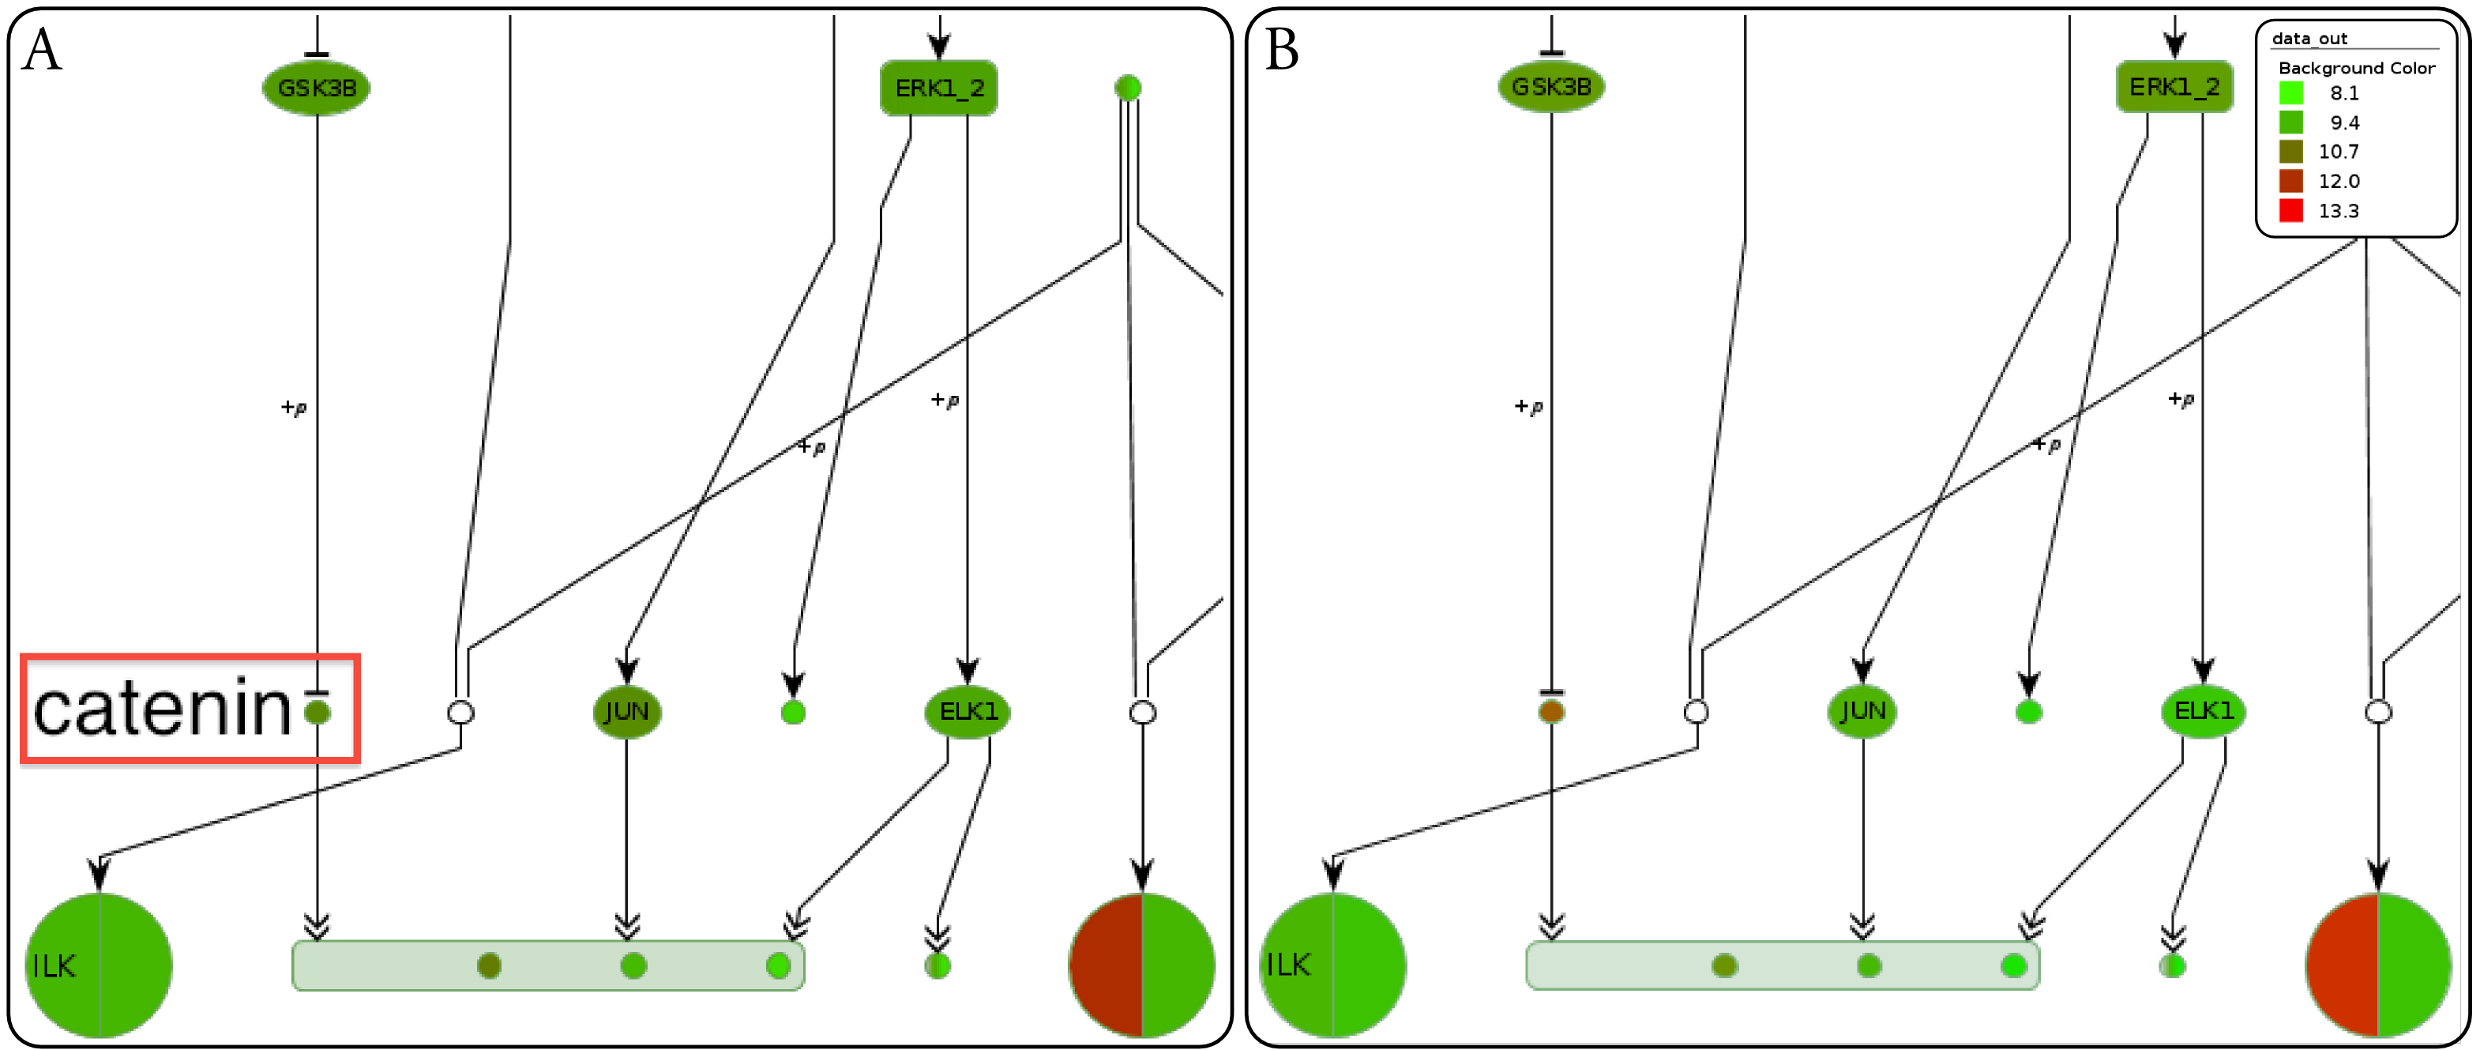
\includegraphics[scale=0.7]{./img/fad_scaled.png}
 % fad_scaled.png: 2480x1050 pixel, 300dpi, 21.00x8.89 cm, bb=0 0 595 252
 \caption{A section from the KEGG pathway \textit{``Focal adhesion''} visualized
by BiNA from the given expression values for the nine tissues. A: in tissue
GSM433783 the protein \textit{catenin} was marked. Its expression value is
comparatively low as can be seen by the green coloring. B: the average
expression values over all remaining samples. For almost every protein they are
the same but only \textit{catenin} is expressed stronger, as illustraed by the
red coloring.}
\label{fig:focAd}
\end{figure}

% 
% 
% \begin{figure}[h]
% \centering
% \begin{minipage}{.4\textwidth}
%   \centering
%   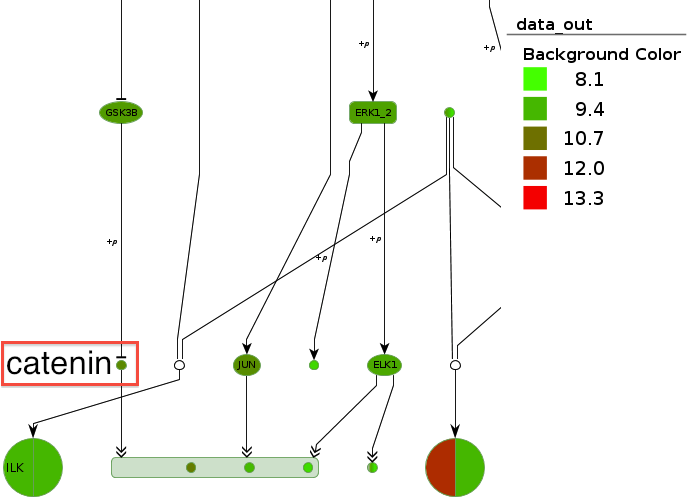
\includegraphics[width=1.2\linewidth]{focal_adhesion83.png}
% \end{minipage}
% \begin{minipage}{.4\textwidth}
%   \centering
%   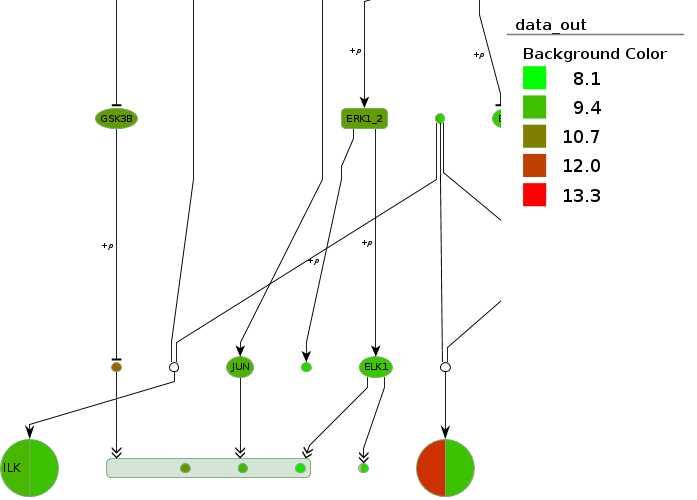
\includegraphics[width=1.2\linewidth]{focal_adhesion_avg.png}
% \end{minipage}
% \caption{A section from the KEGG pathway \textit{``Focal adhesion''} visualized by BiNA from the 
% given expression values for the nine tissues. Left: in tissue GSM433783 the protein \textit{catenin} was marked. Its
% expression value is comparatively low as can be seen by the green coloring. Right: the average expression values over all 
% remaining samples. For almost every protein they are the same but only \textit{catenin} is expressed stronger, as illustraed
% by the red coloring.}
% \label{fig:focAd}
% \end{figure}
